\section{Klassische Kryptographie}
Dieses Kapitel soll eine Zusammenfassung der Grundlagen im Bereich der Kryptografie bieten. Dadurch wird der Einstieg in das Thema Quantenkryptografie erleichtert.
Die Kryptographie ist ein Teilgebiet der Kryptologie, welches sich mit der Absicherung von Daten, beispielsweise der Verschlüsselung von Nachrichten beschäftigt. (Paar, 2016, Vgl. S. 2) 
\subsection{Grundlagen}

Es gibt verschiedene Anwendungsbereiche der Kryptographie. Ein klassisches Einsatzgebiet ist die vertrauliche Kommunikation, also die Geheimhaltung des Nachrichteninhalts. (Paar, 2016, Vgl. S. 6) 
Weitere Anwendungsfälle sind Integrität (Schutz gegen Manipulation), Authentizität (Identitätsnachweis), Verbindlichkeit und Anonymität. (Beutelspacher, 2010, Vgl. S. 3)
\subsection{symmetrische Verschlüsselung}


Die Funktionsweise der symmetrischen Verschlüsselung lässt sich gut anhand eines Beispiels erklären. Alice möchte mit Bob kommunzieren, allerdings gibt es den Angreifer Oskar, der auf dem unsicheren Kanal mithören kann. 


\begin{figure}
    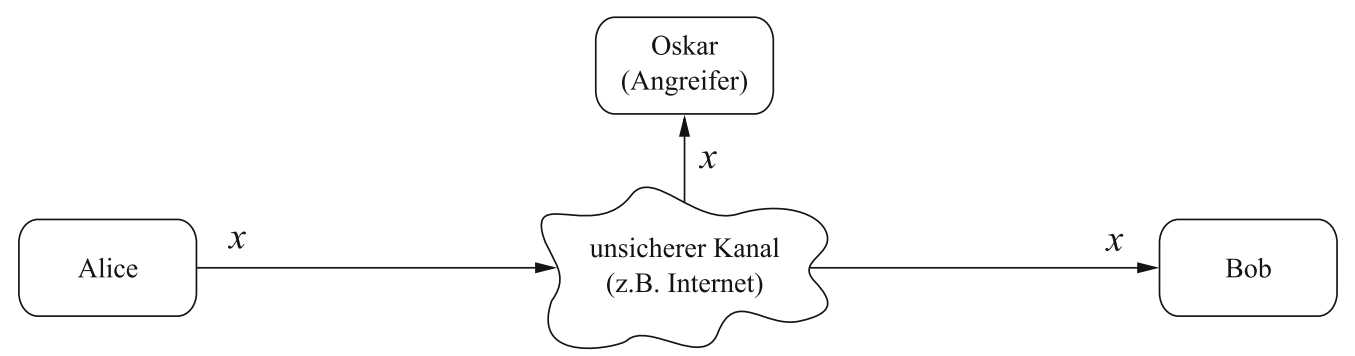
\includegraphics[width=70]{content/bob-alice_unsicherer-kanal.png}
    \caption{Kommunikation über einen unsicheren Kanal mit lauschendem Gegenspieler (Abb. 1.4)}
\end{figure} 

Um die Nachricht zu verschlüsseln, kann Alice die symmetrische Verschlüsselung verwenden. Der Ablauf ist in der folgenden Abbilung dargestellt.
\begin{figure}
    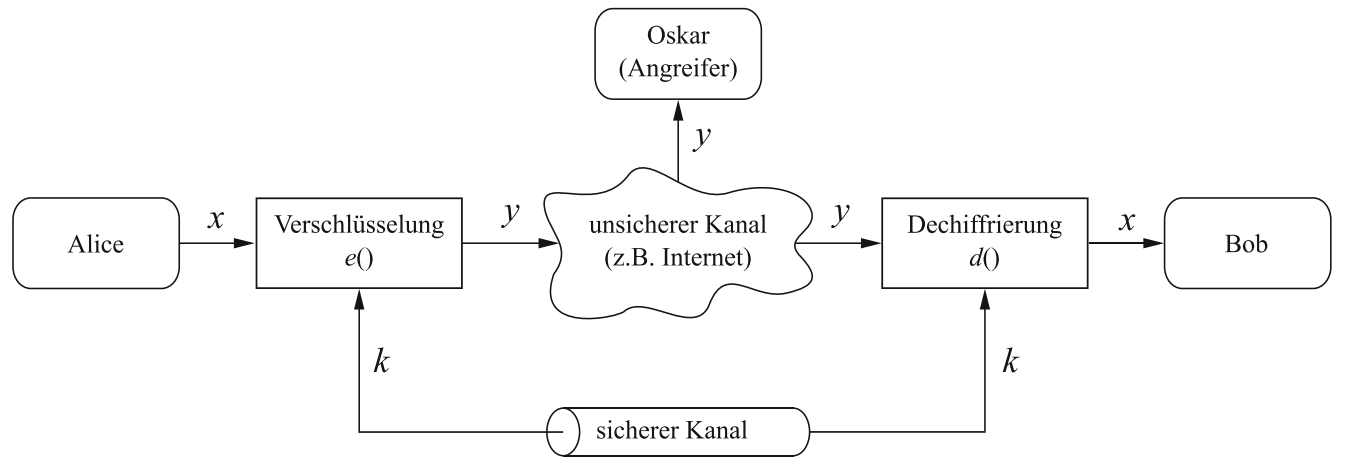
\includegraphics[width=70]{content/bob-alice_sicherer-kanal.png}
    \caption{Verschlüsselung mit symmetrischer Kryptografie (Abb. 1.5)}
\end{figure} 

Alice verschlüsselt ihre Nachricht x mithilfe eines symmetrischen Verfahrens. Das Ergebnis der Verschlüsselung ist das Chiffrat y, das an Bob
geschickt wird, der das Chiffrat wieder entschlüsselt. Das Entschlüsseln ist die inverse Operation der Verschlüsselung. Es wird angenommen, dass das Chiffrat für den Angreifer Oskar wie eine zufällige Zeichenfolge erscheint, es sich demnach um einen starken Verschlüsselungsalgorithmus handelt.\newline

\newline
\subsubsection{Schlüsselübertragung}

Bei der symmetrischen Verschlüsselung muss der Schlüssel über einen sicheren Kanal ausgetauscht werden.\newline
\newline


\subsubsection{Angriffsmöglichkeiten}

Symmentrische Verschlüsselungen können durch vollständige Schlüsselsuche (auch Brute-Force-Angriff genannt) oder eine Frequenz- oder Häufigkeitsanalyseangegriffen werden. (Beutelspacher, 2010, Vgl. S. 7 - 9)\newline
\newline


\subsection{asymmetrische Verschlüsselung}






\subsection{Vergleich Symmetrische-Asymmetrische Algorithmen}
S.114


\subsection{Auswirkungen von Quantencomputern auf die Kryptografie}
"Wenn Quantencomputer eines Tages existieren sollten, würden sie die effektive Schlüssellänge
symmetrischer Chiffren halbieren. Die optimistischsten Prognosen gehen momentan, d. h. 2016,
davon aus, dass Quantenrechner frühestens 2030 zur Verfügung stehen werden, und es gibt viele
Fachleute, die Zeiträume von 30–50 Jahren für realistischer halten. Man beachte, dass alle heutzutage verwendeten asymmetrischen Algorithmen mit Quantencomputern gebrochen werden können, unabhängig von der gewählten Schlüssel" (s. 26 hinweis quantencomputer)

\newline \newline
\exercise[type=multipleChoice]{
    \question{Frage: Was ist ein Quantencomputer?}
    \possibleAnswers{
        \item 1) Recheneinheiten in Smartphones werden als Quantencomputer bezeichnet.
        \item 2) Computer, die auf Basis quantenmechanischer Zustände arbeiten.
    }
    \result{2}
}




\newline \newline
\subsection{Quellen}

[Beutelspacher 2010] Beutelspacher, Albrecht, et al. Kryptografie in Theorie Und Praxis: Mathematische Grundlagen Für Internetsicherheit, Mobilfunk Und Elektronisches Geld. Vieweg + Teubner, 2010. 
\newline
[Paar 2016] Paar, Christof, and Jan Pelzl. Kryptografie verständlich: Ein Lehrbuch für Studierende Und Anwender. Springer Berlin Heidelberg, 2016. 